\subsection{Program-incumbent promotion margins}\label{app:program-promotion-margins}

\Cref{fig:program-promotion-margins} extends the retained program-promotion
record to the run's last event. Each margin compares programs in one
context; the admitted-event journal supplies no proposal-attempt denominator.

\begin{figure}[!tb]
  \centering
  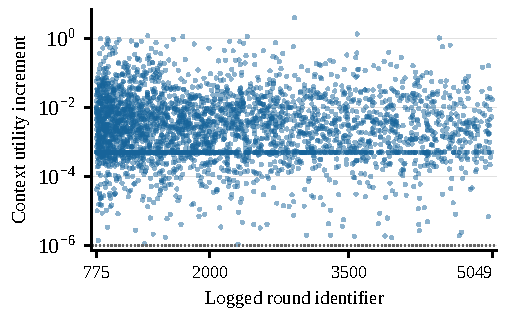
\includegraphics[width=\linewidth]{figures/fig_program_promotion_margins.pdf}
  \caption{\textbf{Program-incumbent promotions have unequal utility margins.}
  All \num{3529} ordinary promotion records in rounds 775--5049; the
  last is at round 5047 (11:13 UTC, 4 November 2026). Each point
  subtracts old from new logged utility in its own training context;
  larger is better. Pre-775 warm-up and historical admissions are
  excluded. Logarithmic axis; dotted line: the $10^{-6}$ admission margin.
  Admission requires positive increments. These cannot be summed
  across contexts or interpreted as proposal success, adapter improvement
  or writer learning. Scope: \cref{sec:method-status}.}
  \label{fig:program-promotion-margins}
\end{figure}
